\section{Evaluation}
\label{sec:lego:results}

This section presents the performance evaluation of \lego\ using micro- and macro-benchmarks and two unmodified real applications.
We also quantitatively analyze the failure rate of \lego.
We ran all experiments on a cluster of 10 machines, each with two Intel Xeon CPU E5-2620 2.40GHz
processors, 128 GB DRAM, and one 40 Gbps Mellanox ConnectX-3 InfiniBand network adapter;
a Mellanox 40 Gbps InfiniBand switch connects all of the machines. 
The Linux version we used for comparison is v4.9.47.

\subsection{Micro- and Macro-benchmark Results}
\noindent{\textit{\uline{Network performance.}}}
Network communication is at the core of \lego' performance.
Thus, we evaluate \lego' network performance first before evaluating \lego\ as a whole.
Figure~\ref{fig-net-latency} plots the average latency of sending messages with socket-over-InfiniBand (Linux-IPoIB) in Linux,
\lego' implementation of socket on top of InfiniBand (LegoOS-Sock-o-IB), and \lego' implementation of RPC over InfiniBand (LegoOS-RPC-IB).
\lego\ uses LegoOS-RPC-IB for all its internal network communication across components and uses LegoOS-Sock-o-IB for 
all application-initiated socket network requests.
Both \lego' networking stacks significantly outperform Linux's.

\noindent{\textit{\uline{Memory performance.}}}
Next, we measure the performance of \mcomponent\ using a multi-threaded user-level micro-benchmark. 
In this micro-benchmark, each thread performs one million sequential 4\KB\ memory loads in a heap.
We use a huge, empty \excache\ (32\GB) to run this test, 
so that each memory access can generate an \excache\ (cold) miss and go to the \mcomponent.

Figure~\ref{fig-iops-memory} compares \lego' \mcomponent\ performance 
with Linux's single-node memory performance using this workload.
We vary the number of per-\mcomponent\ worker threads from 1 to 8 
with one and two \mcomponent{}s (only showing representative configurations in Figure~\ref{fig-iops-memory}).
In general, using more worker threads per \mcomponent\ and using more \mcomponent{}s both improve throughput when an application has high parallelism,
but the improvement largely diminishes after the total number of worker threads reaches four.
%but using 4 worker threads can already saturate the performance.
We also evaluated the optimization technique in \S~\ref{sec:lego:zerofill} ({\em p-local} in Figure~\ref{fig-iops-memory}).
As expected, bypassing \mcomponent\ accesses with p-local lines significantly 
improves memory access performance.
The difference between p-local and Linux demonstrates the overhead of trapping to \lego\ kernel and setting up \excache.

\noindent{\textit{\uline{Storage performance.}}}
To measure the performance of \lego' storage system, we ran a single-thread micro-benchmark 
that performs sequential and random 4\KB\ read/write to a 25\GB\ file on a Samsung PM1725s NVMe SSD (the total amount of data accessed is 1\GB).
For write workloads, we issue an {\em fsync} after each {\em write} to test the performance of writing all the way to the SSD.

Figure~\ref{fig-iops-storage} presents the throughput of this workload on \lego\ and on single-node Linux.
For \lego, we use one \mcomponent\ to store the buffer cache of this file and initialize the buffer cache to empty
so that file I/Os can go to the \scomponent\ (Linux also uses an empty buffer cache).
Our results show that Linux's performance is determined by the SSD's read/write bandwidth.
\lego' random read performance is close to Linux, since network cost is relatively low compared to the SSD's random read performance.
With better SSD sequential read performance, network cost has a higher impact.
\lego' write-and-fsync performance is worse than Linux because
\lego\ requires one RTT between \pcomponent\ and \mcomponent\ to perform write 
and two RTTs (\pcomponent\ to \mcomponent, \mcomponent\ to \scomponent) for fsync.

{
\begin{figure*}[t]
\begin{center}
\centerline{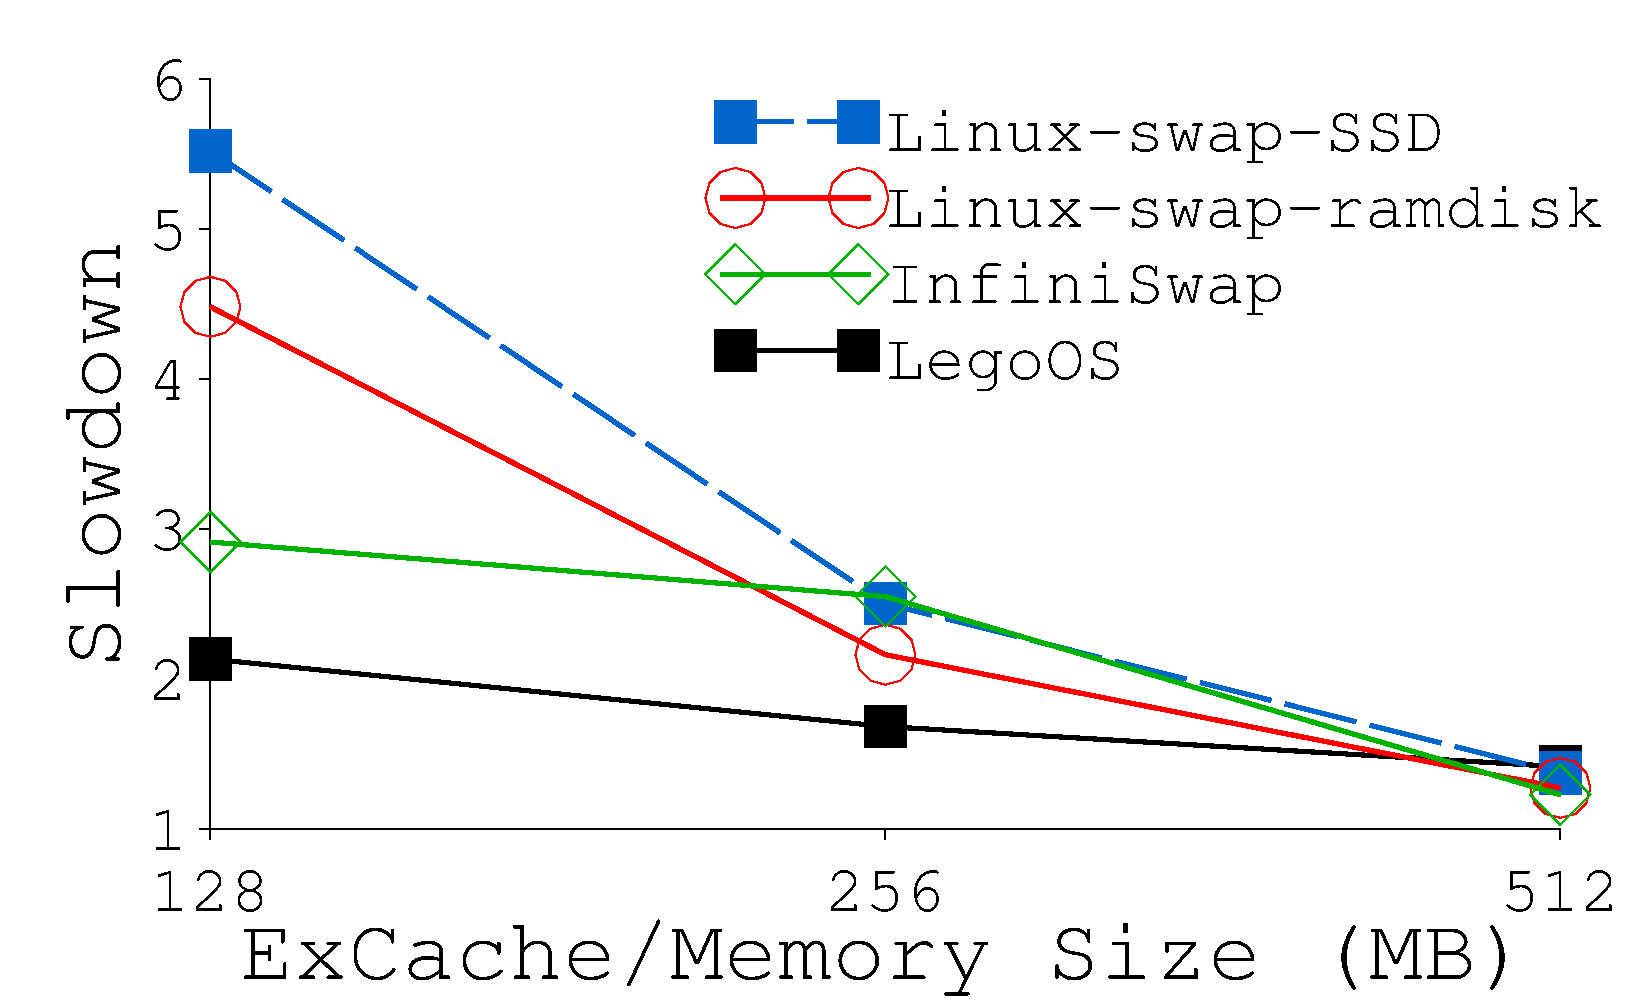
\includegraphics[width=0.5\textwidth]{lego/Figures/g_plot_LEGO_tf4.pdf}}
\caption[TensorFlow Performance.]{TensorFlow Performance.}
\label{fig-tf4}
\end{center}
\end{figure*}
}
{
\begin{figure*}[th]
\begin{center}
\centerline{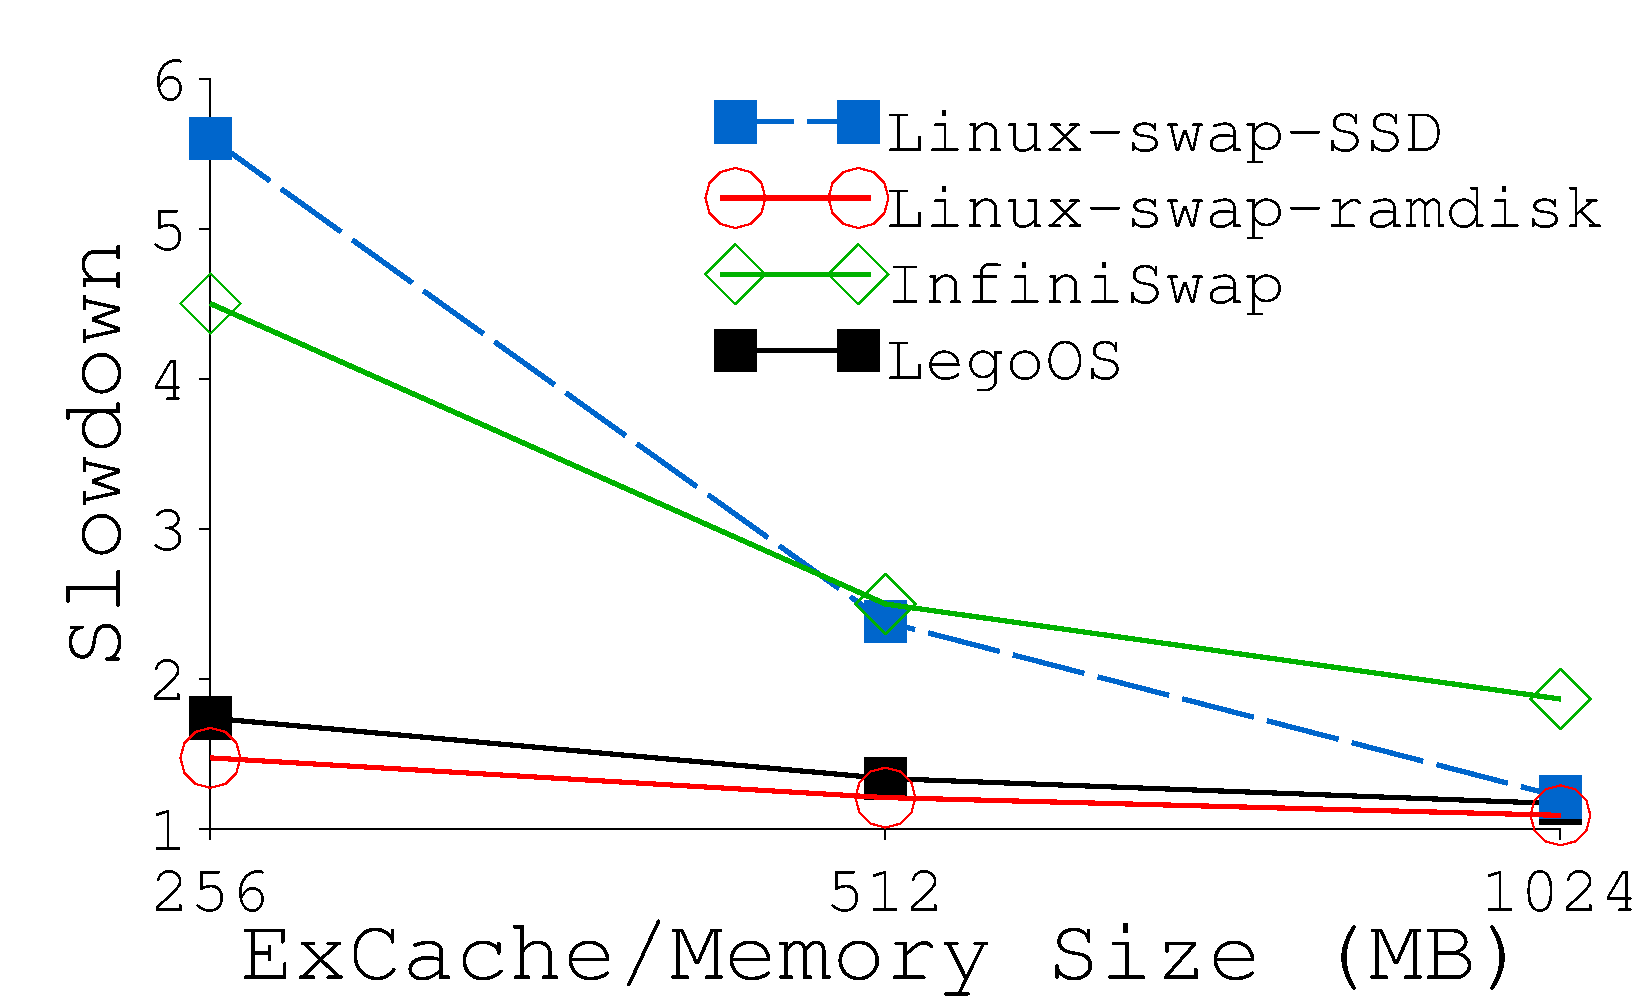
\includegraphics[width=0.5\textwidth]{lego/Figures/g_plot_LEGO_phoenix.pdf}}
\caption{Phoenix Performance.}{Phoenix Performance.}
\label{fig-phoenix}
\end{center}
\end{figure*}
}
{
\begin{figure*}[th]
\begin{center}
\centerline{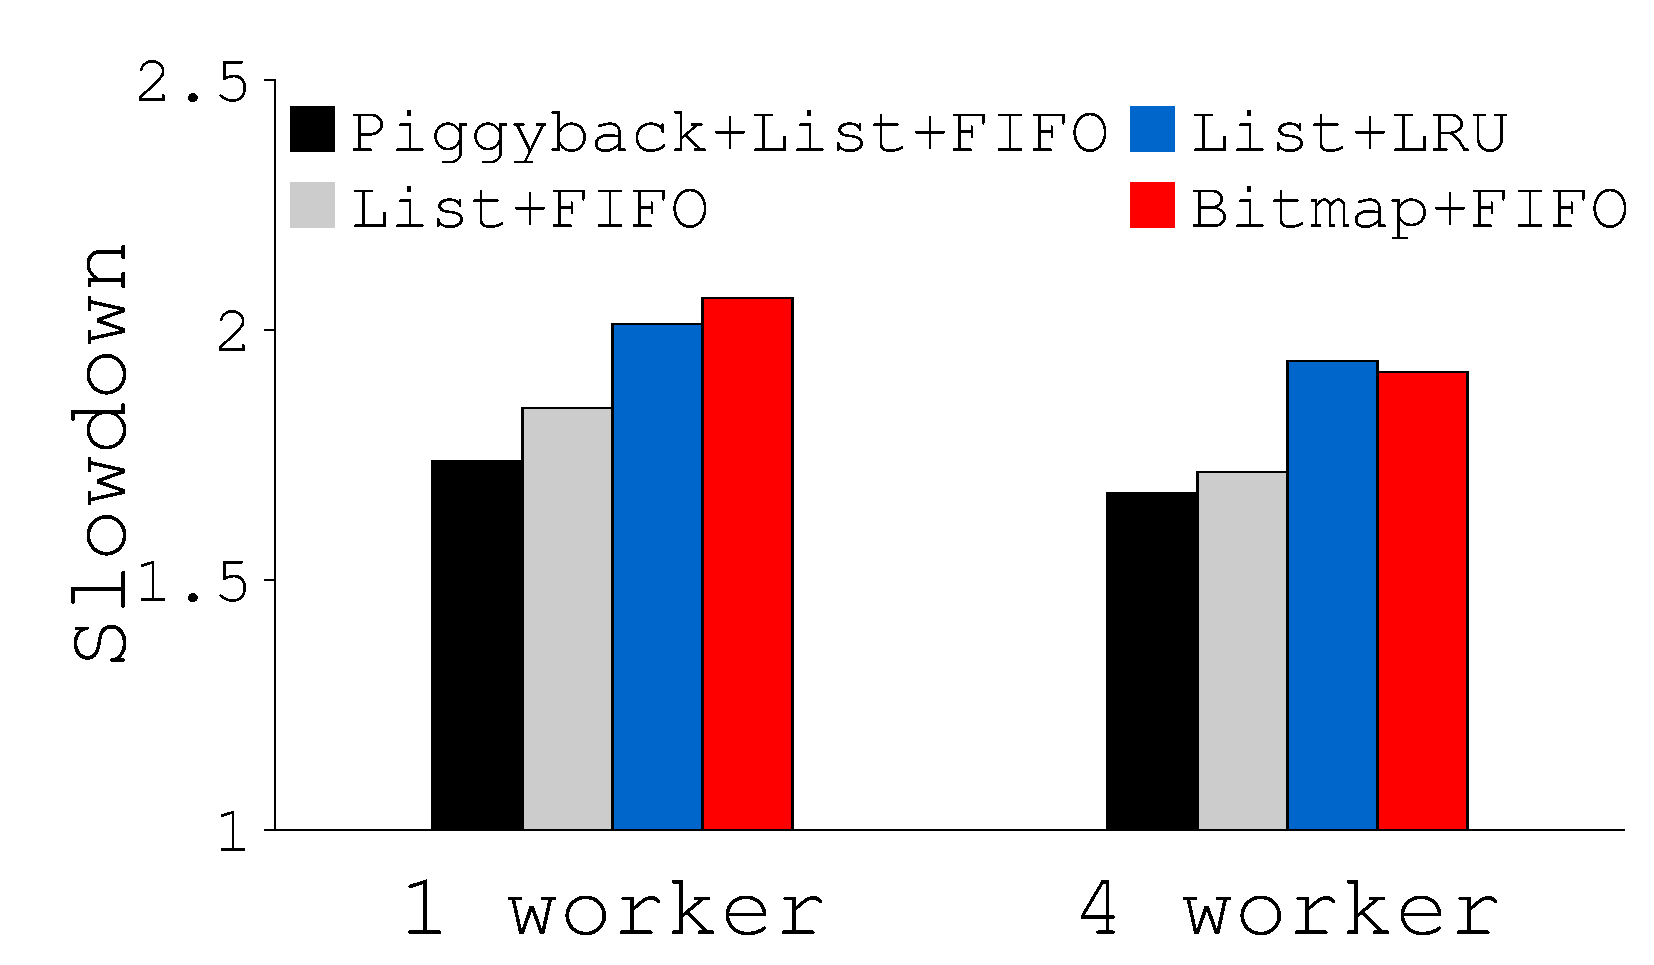
\includegraphics[width=0.5\textwidth]{lego/Figures/g_plot_LEGO_excache_tech.pdf}}
\caption{ExCache Management.}{ExCache Management.}
\label{fig-excache-opt}
\end{center}
\end{figure*}
}
{
\begin{figure*}[th]
\begin{center}
\centerline{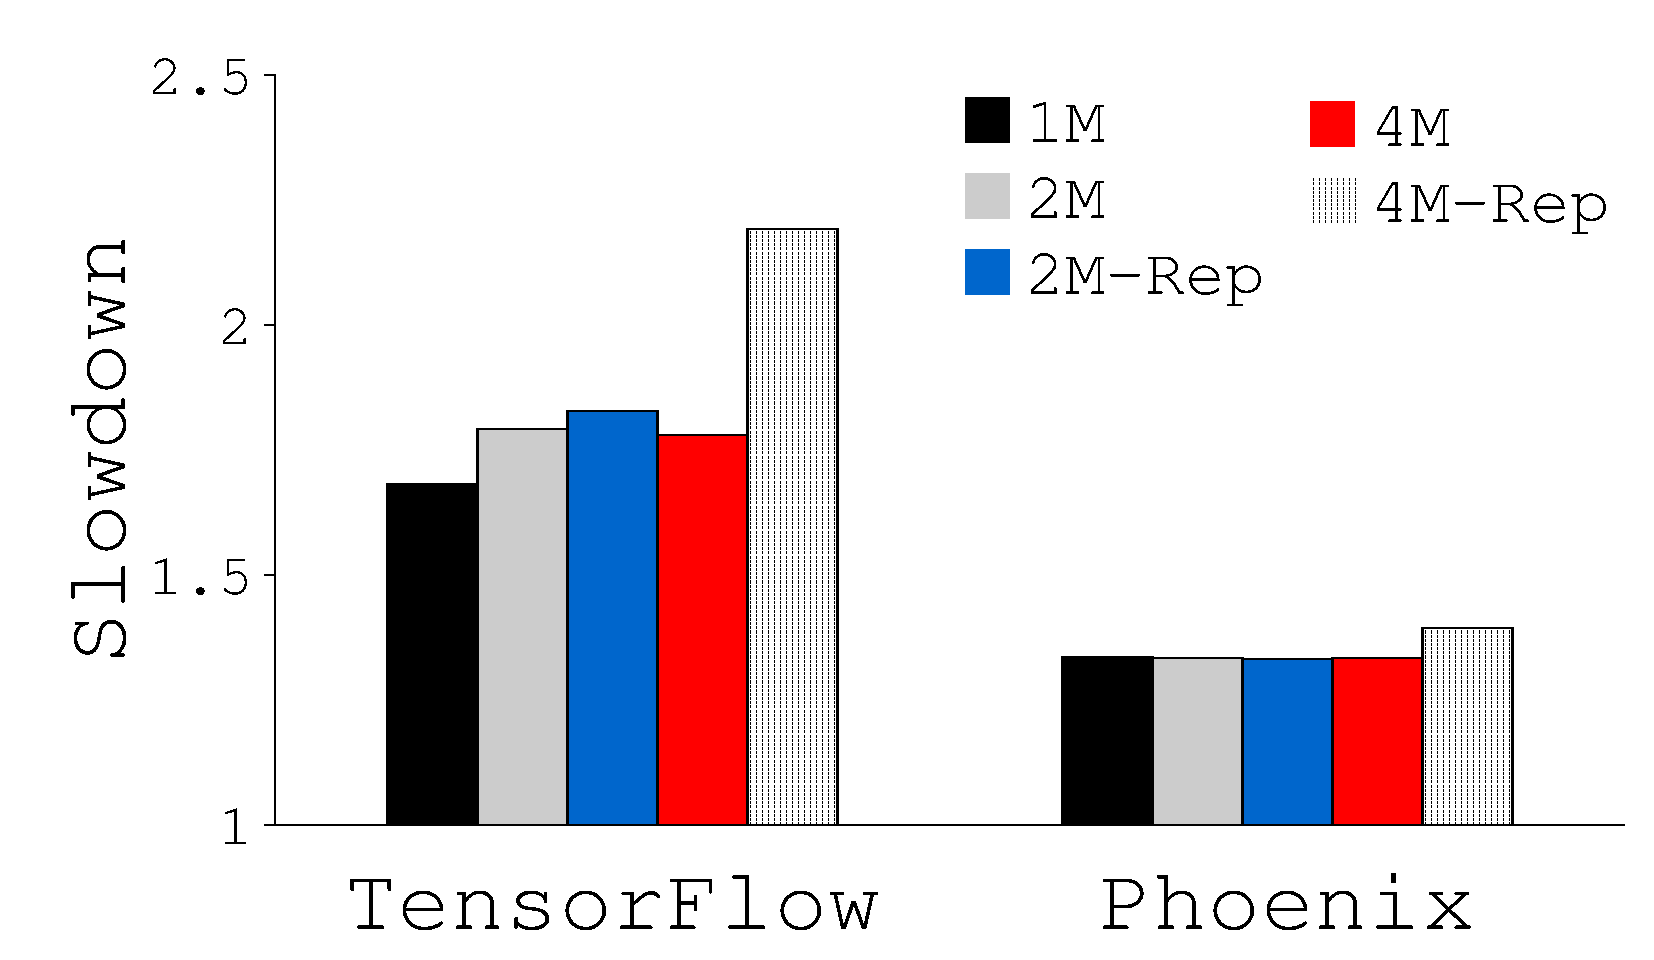
\includegraphics[width=0.5\textwidth]{lego/Figures/g_plot_LEGO_number_memory_rep.pdf}}
\caption[Memory Config.]{Memory Config.}
\label{fig-mem-rep}
\end{center}
\end{figure*}
}
\noindent{\textit{\uline{PARSEC results.}}}
We evaluated \lego\ with a set of workloads from the PARSEC benchmark suite~\cite{PARSEC},
including BlackScholes, Freqmine, and StreamCluster.
These workloads are a good representative of compute-intensive datacenter applications, 
ranging from machine-learning algorithms to streaming processing ones.
Figure~\ref{fig-parsec} presents the slowdown of \lego\ 
over single-node Linux with enough memory for the entire application working sets.
\lego\ uses one \pcomponent\ with 128\MB\ \excache,
one \mcomponent\ with one worker thread, and one \scomponent\ for all the PARSEC tests.
For each workload, we tested one and four workload threads.
StreamCluster, a streaming workload, performs the best because of its 
batching memory access pattern (each batch is around 110\MB).
BlackScholes and Freqmine perform worse because of their larger working sets (630\MB\ to 785\MB).
\lego\ performs worse with higher workload threads, 
because the single worker thread at the \mcomponent\ becomes the bottleneck to achieving higher throughput.
%This result suggests that stream processing is a good fit to \lego.
%Finally, for these PARSEC workloads, the number of \mcomponent s have no or small effects.

\subsection{Application Performance}
\label{sec:appresults}
We evaluated \lego' performance with two real, unmodified applications, 
TensorFlow~\cite{TensorFlow} and Phoenix~\cite{Ranger07-HPCA}, a single-node multi-threaded implementation of MapReduce~\cite{DeanEtAl04-MapReduce}.
TensorFlow's experiments use the Cifar-10 dataset~\cite{CIFAR-DS} and Phoenix's use a Wikipedia dataset~\cite{Wiki-DS}.
Unless otherwise stated, the base configuration used for all TensorFlow experiments
is 256\MB\ 64-way \excache, one \pcomponent, one \mcomponent, and one \scomponent.
The base configuration for Phoenix is the same as TensorFlow's with the exception that the base \excache\ size is 512\MB.
The total amount of virtual memory addresses touched in TensorFlow is 4.4\GB\ (1.75\GB\ for Phoenix).
The total working sets of the TensorFlow and Phoenix execution are 0.9\GB\ and 1.7\GB.
Our default \excache\ sizes are set as roughly 25\% of total working sets.
We ran both applications with four threads.

\noindent{\textit{\uline{Impact of \excache\ size on application performance.}}}
Figures~\ref{fig-tf4} and \ref{fig-phoenix} plot the TensorFlow and Phoenix run time comparison across 
\lego, a remote swapping system (InfiniSwap~\cite{GU17-NSDI}), 
a Linux server with a swap file in a local high-end NVMe SSD, 
and a Linux server with a swap file in local ramdisk.
All values are calculated as a slowdown to running the applications on a Linux server that have enough local resources (main memory, CPU cores, and SSD).
For systems other than \lego, we change the main memory size to the same size of \excache\ in \lego, with rest of the memory on swap file. 
With around 25\% working set, \lego\ only has a slowdown of 1.68\x\ and 1.34\x\ for TensorFlow and Phoenix
%of incurs the overhead of TensorFlow and Phoenix on \lego\ are 
compared to a monolithic Linux server that can fit all working sets in its main memory.

\lego' performance is significantly better than swapping to SSD and to remote memory 
largely because of our efficiently-implemented network stack, simplified code path compared with Linux paging subsystem,
and the optimization technique proposed in \S\ref{sec:lego:zerofill}.
Surprisingly, it is similar or even better than swapping to local memory, even when \lego' memory accesses are across network.
This is mainly because ramdisk goes through buffer cache and incurs memory copies between the buffer cache and the in-memory swap file.

\lego' performance results are not easy to achieve and we went through rounds of design and implementation refinement.
Our network stack and RPC optimizations yield a total improvement of up to 50\%.
For example, we made all RPC server (\mcomponent's) replies {\em unsignaled} to save \mcomponent' processing time
and to increase its request handling throughput.
Another optimization we did is to piggy-back dirty cache line flush and cache miss fill into one RPC.
The optimization of the first anonymous memory access (\S\ref{sec:lego:zerofill}) improves \lego' performance further by up to 5\%.

\noindent{\textit{\uline{\excache\ management.}}}
Apart from its size, how an \excache\ is managed can also largely affect application performance.
We first evaluated factors that could affect \excache\ hit rate and found that higher associativity improves hit rate
but the effect diminishes when going beyond 512-way.
We then focused on evaluating the miss cost of \excache, since the miss path is handled by \lego\ in our design.
We compare the two eviction policies \lego\ supports (FIFO and LRU),
two implementations of finding an empty line in an \excache\ set (linearly scan a free bitmap and fetching the head of a free list),
and one network optimization (piggyback flushing a dirty line with fetching the missing line).

Figure~\ref{fig-excache-opt} presents these comparisons with one and four \mcomponent\ worker threads. 
All tests run the Cifar-10 workload on TensorFlow with 256\MB\ 64-way \excache, one \mcomponent, and one \scomponent.
Using bitmaps for this \excache\ configuration is always worse than using free lists
because of the cost to linearly scan a whole bitmap,
and bitmaps perform even worse with higher associativity.
Surprisingly, FIFO performs better than LRU in our tests, even when LRU utilizes access locality pattern.
We attributed LRU's worse performance to the lock contention it incurs;
the kernel background thread sweeping the \excache\ locks an LRU list when adjusting the position of an entry in it,
while \excache\ miss handler thread also needs to lock the LRU list to grab its head.
Finally, the piggyback optimization works well and the combination of FIFO, free list, and piggyback yields the best performance.

\noindent{\textit{\uline{Number of \mcomponent{}s and replication.}}}
Finally, we study the effect of the number of \mcomponent s and memory replication.
Figure~\ref{fig-mem-rep} plots the performance slowdown as the number of \mcomponent s increases from one to four.
Surprisingly, using more \mcomponent{}s lowers application performance by up to 6\%.
This performance drop is due to the effect of \excache\ piggyback optimization. 
When there is only one \mcomponent, flushes and misses are all between the \pcomponent\ and this \mcomponent,
thus enabling piggyback on every flush.
%the \mcomponent\ to be flushed to is always the  to fetch the missing page from.
However, when there are multiple \mcomponent{}s, \lego\ can only perform piggyback when flushes and misses are to the same \mcomponent.
%this is not true anymore. Essentially,
%multiple \mcomponent s case will involve more network RPC than one \mcomponent\ case.

We also evaluated \lego' memory replication performance in Figure~\ref{fig-mem-rep}.
Replication has a performance overhead of 2\% to 23\% (there is a constant 1\MB\ space overhead to store the backup log).
\lego\ uses the same application thread to send the replica data to the backup \mcomponent\ and then 
to the primary \mcomponent, resulting in the performance lost. 
%The performance overhead is a result of 
%We also tested synchronous replication where foreground waits for the write back of backup memory log.
%The synchronous replication scheme has an overhead of 1.2\%.

\noindent{\textit{\uline{Running multiple applications together.}}}
All our experiments so far run only one application at a time.
Now we evaluate how multiple applications perform when running them together on a \lego\ cluster.
We use a simple scenario of running one TensorFlow instance and one Phoenix instance together in two settings:
1) two \pcomponent{}s each running one instance, both accessing one \mcomponent (2P1M),
and 2) one \pcomponent\ running two instances and accessing two \mcomponent{}s (1P2M).
Both settings use one \scomponent. Figure~\ref{fig-multiapp} presents the runtime slowdown results.
We also vary the number of \mcomponent\ worker threads for the 2P1M setting (4 and 8 workers)
and the amount of \excache\ for the 1P2M setting (1\GB\ and 0.5\GB).
With 2P1M, both applications suffer from a performance drop
because their memory access requests saturate the single \mcomponent.
Using more worker threads at the \mcomponent\ improves the performance slightly.
%due to burst memory access requests from both applications resulting much higher queuing delay in the \mcomponent.
For 1P2M, application performance largely depends on \excache\ size, similar to our findings with single-application experiments.

{
\begin{figure*}[t]
\begin{center}
\centerline{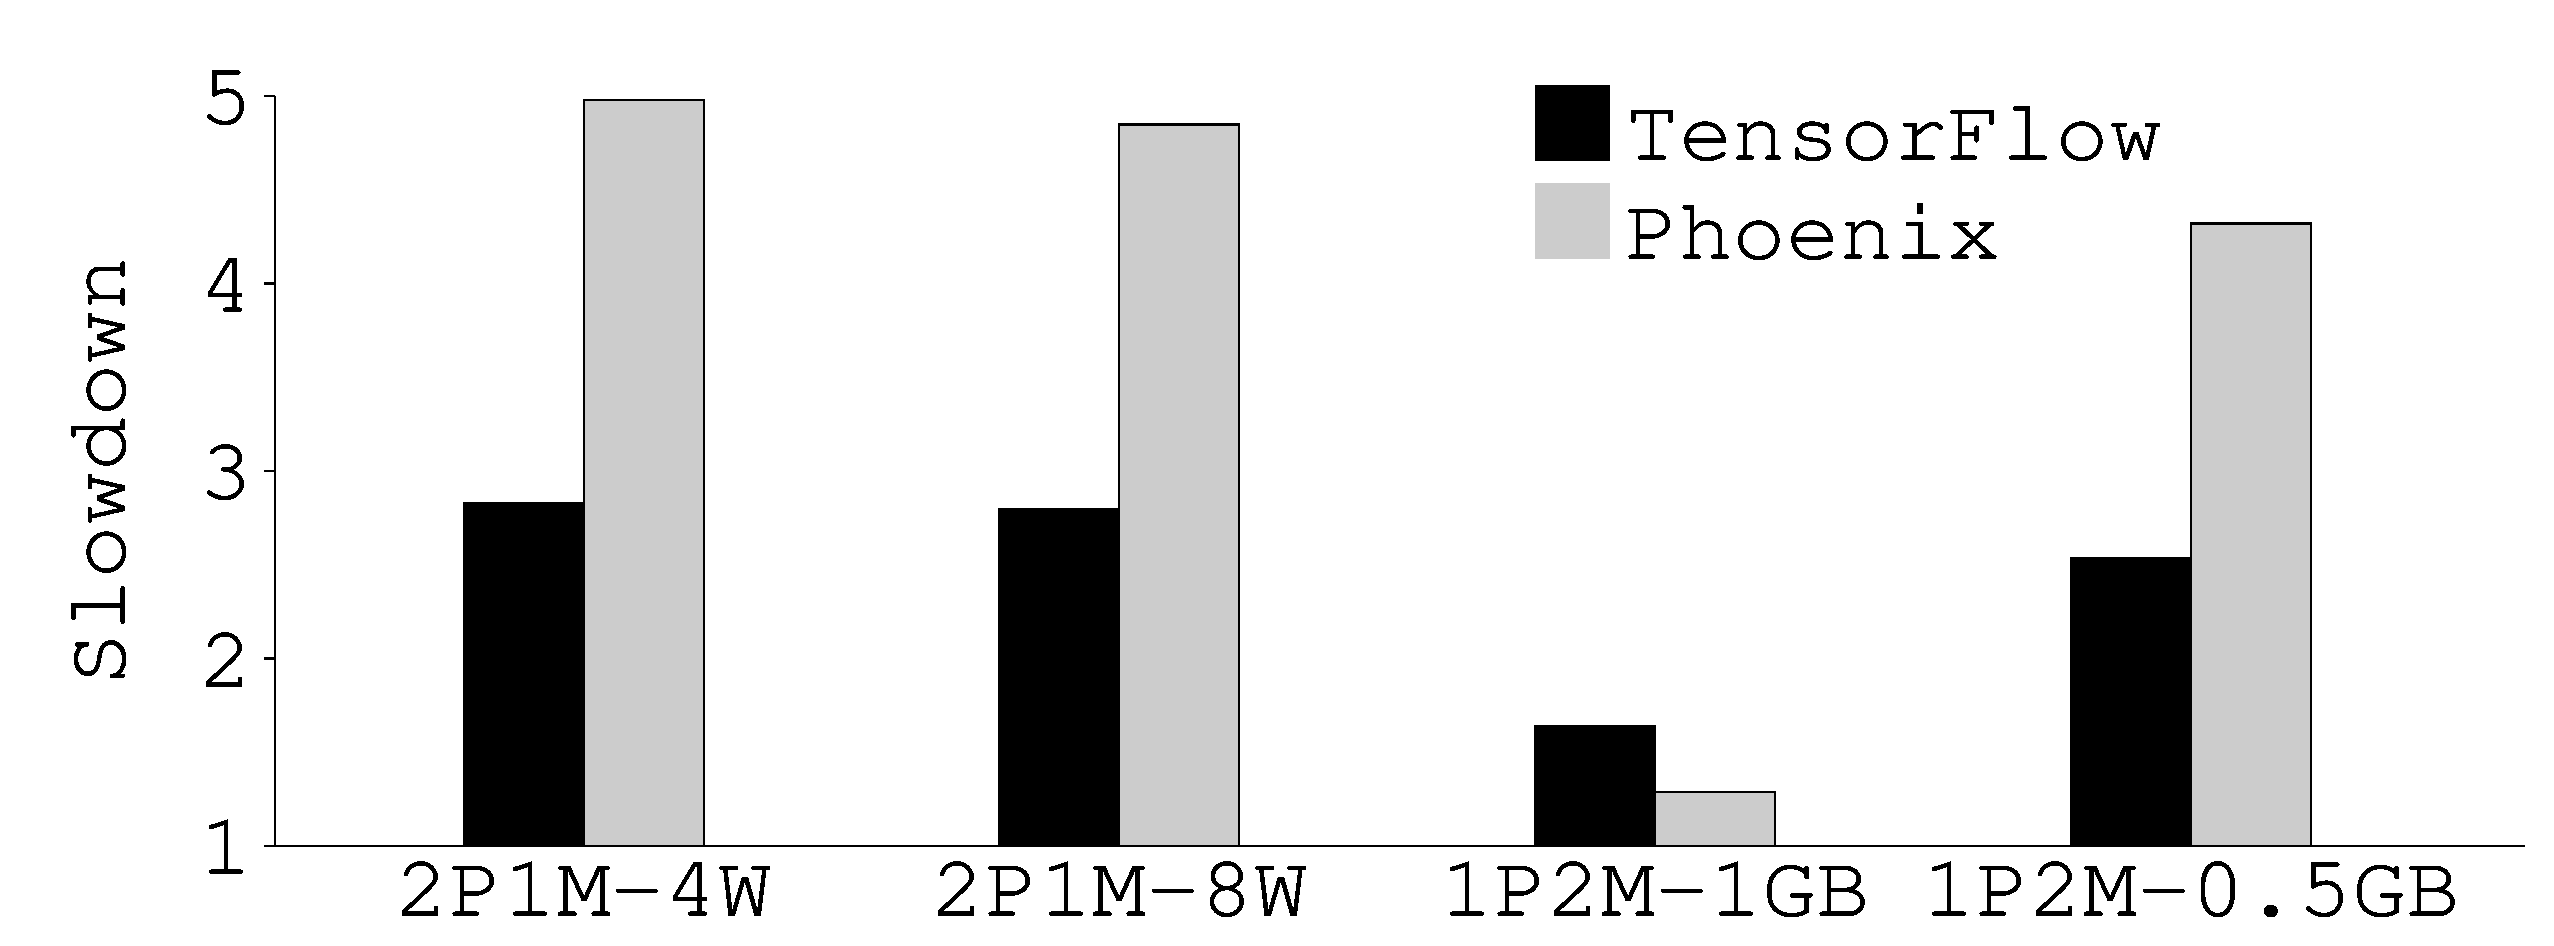
\includegraphics[width=0.6\textwidth]{lego/Figures/g_plot_LEGO_multiapp.pdf}}
\caption[Multiple Applications.]{Multiple Applications.}
\label{fig-multiapp}
\end{center}
\end{figure*}
}
%s to two applications running on same \pcomponent, 0.5G Excahce, being 19.7\% of resident memory, results
%much higher cache conflicts and evictions, furthermore reflected by 3-4 times slowdown in runtime. Meanwhile,
%1\GB\ \excache, 39.4\% of resident memory, reveals a better performance than the former.

\if 0
\subsection{Resource Packing Analysis}
\label{sec:cost}
A key advantage of a \lego\ cluster is its better resource packing compared to a monolithic cluster.
We provide a quantitative analysis of this benefits using the Google cluster trace~\cite{GoogleTrace}.
This cluster only runs VMs and the trace reports the amount of physical machines used to run the VMs 
in a 29-day period. 
The trace also provides the total amount of CPU and memory in each physical machine
and the amount of CPU and memory used by each VM.
With this set of information, we calculated the CPU and memory utilization of the whole Google cluster.

We calculate the amount of total memory and total CPU needed for a \lego\ cluster separately.
For memory, since \lego\ can freely allocate memory from any \mcomponent{}s and the allocation is performed on demand, 
we simply use the estimation of total memory required being {\small{$1+RepOvhd$}} of total memory used,
where {\small{$RepOvhd$}} is the space overhead to store the backup log for each \mcomponent.
The estimation of \lego' CPU usage is more complex.
Since \lego\ cannot split a process across \pcomponent{}s and the trace does not provide information of 
processes within a VM, we simply treat one VM as the unit of allocation.
We perform a further estimation by using a first-fit allocation algorithm to assign VMs to \pcomponent{}s 
based on available cores of \pcomponent{}s.

\fixme{will continue analysis after power outage}
\fi

{
\begin{table*}[th]\footnotesize
\begin{center}
\begin{tabular}{ l || c | c | c | c | c | c || c | c}
 & Processor & Disk & Memory  & NIC & Power & Other & Monolithic & \lego\ \\
\hline
%Unit Cost & \$6500 & \$530 & \$760 & \$360 & \$380 &\$320 & \$7400 & N/A \\
%Monolithic & 100 & (200) & (400) & (100) & (100) & 100 & 3  & \$704,200\\
%Disaggregation & 0 & 100 & 200 + 50 & 0 & 100 & 125 & 4 & \$350,600 \\

MTTF (year) & 204.3 & 33.1 & 289.9 & 538.8 & 100.5 & 27.4 & 5.8 & 6.8 - 8.7 \\
%MTTF  & &&&&&& \\

\end{tabular}
\end{center}
\vspace{-0.2in}
\mycaption{tbl-failure}{Mean Time To Failure Analysis.}
{
MTTF numbers of devices (columns 2 to 7) are obtained from~\cite{Failure-Disk-FAST07}
and MTTF values of monolithic server and \lego\ are calculated using the per-device MTTF numbers.
%Unit: year.
%MTTPF: Mean Time To Permanent (hardware) Failure, MTTF: Mean Time To (all types of hardware) Failure.
%Per-device MTTF used to calculate MTTPF are collected from Table 3 in \cite{Failure-Disk-FAST07}.
%Processor failure includes the failure of CPU, fan, and CPU heat sink (for both monolithic server and Lego).
}
%\vspace{-0.1in}
\end{table*}
%\vspace{-0.1in}
}


\subsection{Failure Analysis}
\label{sec:lego:failure-results}
Finally, we provide a qualitative analysis on the failure rate of a \lego\ cluster compared to a monolithic server cluster.
Table~\ref{tbl-failure} summarizes our analysis.
To measure the failure rate of a cluster, we use the metric Mean Time To (hardware) Failure (MTTF), 
the mean time to the failure of a server in a monolithic cluster
or a component in a \lego\ cluster.
Since the only real per-device failure statistics we can find are
the mean time to hardware replacement in a cluster~\cite{Failure-Disk-FAST07},
the MTTF we refer to in this study indicates the mean time to the type of 
hardware failures that require replacement.
Unlike traditional MTTF analysis, we are not able to include transient failures.
%MTTF indicates the frequency of hardware replacement in a cluster.

To calculate MTTF of a monolithic server, we first obtain the replacement frequency of different hardware devices in a server
(CPU, memory, disk, NIC, motherboard, case, power supply, fan, CPU heat sink, and other cables and connections)
from the real world (the COM1 and COM2 clusters in \cite{Failure-Disk-FAST07}).
For \lego, we envision every component to have a NIC and a power supply, 
and in addition, a \pcomponent\ to have CPU, fan, and heat sink, an \mcomponent\ to have memory, and an \scomponent\ to have a disk.
We further assume both a monolithic server and a \lego\ component to fail when any hardware devices in them fails
and the devices in them fail independently.
Thus, the MTTF can be calculated using the harmonic mean ({\em HM}) 
of the MTTF of each device.

\vspace{-0.05in}

\begin{small}
\begin{equation}
MTTF = \frac{HM_{i=0}^n(MTTF_i)}{n}
\end{equation}
\end{small}

\vspace{-0.05in}

\noindent where $n$ includes all devices in a machine/component. 

Further, when calculating MTTF of \lego, we estimate the amount of components needed in \lego\ 
to run the same applications as a monolithic cluster.
Our estimated worst case for \lego\ is to use the same amount of hardware devices 
(\ie, assuming same resource utilization as monolithic cluster).
\lego' best case is to achieve full resource utilization 
and thus requiring only about half of CPU and memory resources 
(since average CPU and memory resource utilization in monolithic server clusters is around 50\%~\cite{GoogleTrace,AliTrace}).

With better resource utilization and simplified hardware components (\eg, no motherboard),
\lego\ improves MTTF by 17\% to 49\% compared to an equivalent monolithic server cluster.

\if 0
Best case:
\begin{equation}
MTTF_{Lego} = \frac{HM(MTTF_P, MTTF_M, MTTF_S)}{3}
\end{equation}

Worst case:
\begin{equation}
MTTF_{Lego} = \frac{HM(MTTF_P/2, MTTF_M/2, MTTF_S)}{3}
\end{equation}
\fi

